\chapter{Scalable Flow Classification}\label{chap:seidr}

% \section{Motivation}
% \section{Sei\dh{}r Histograms}
% \subsection{Algorithm}
% \subsection{Packet Generation on PSA}
% \section{Use case: TCP CCA Detection}
% \subsection{Observable Differences}
% \subsection{Investigating the BBR Algorithm}
% \section{Methodology}
% \subsection{Testing Environments}
% \subsection{Data Collection/Generation}
% \subsection{ML Model Architecture}
% \section{Evaluation}
% \subsection{Device Memory Costs}
% \subsection{Bandwidth Costs}
% \subsection{CCA Detection Accuracy and Costs}

%?? Problem statement: damn, all this ML is cool
%?? We can do cool real-time analysis of operational Internet traffic
%?? What do we do if we need more complex ML models: i.e., need to use LSTMs, or complex CNNs because we need to make use of complex temporal or structural features of data? We still need to get it to host machonies.
%?? Okay... but in that case, how can we reduce data so that PPS and Gbps of data don't overwhelm the host, or that we lose lots of said data and make poor decisions when we have many (or very fast) flows?
%
%?? supposing we have analyses which cannot be offloaded: too long-reaching (needing LSTMs or CNNs w/ todays hardware)

The \gls{acr:ml} techniques we have considered so far are powerful and effective and, with some amount of work, many can be ported to fit quite neatly into \gls{acr:pdp} hardware.
Between the existing literature and the novel additions demonstrated until now, we have a toolkit of models and runtime techniques that neatly runs the gamut of \gls{acr:ddn} use cases' needs.
Real-time analysis of operational Internet, \gls{acr:wan}, and data centre traffic using granular, device-local state is that much more feasible because of their development.
This can be through accurate flow characterisation (or classification), which can drive intrusion detection, prioritisation of traffic for certain customers, providing path-diversity, as well as marking the \gls{acr:qos} of various users and protocols~\parencite{DBLP:journals/ccr/BernailleTASS06,DBLP:conf/lisa/Roesch99}; some of these use cases are feasible even with the sampled, imprecise \unit{\micro\second} and \unit{\milli\second}-level data of sFlow, Netflow, and IPFIX~\parencite{rfc7011,rfc3954}.
We have seen through \cref{sec:network-monitoring} the sorts of advances in dataplane monitoring which will allow us to further develop traffic analytics and classifiers, such as precise \unit{\nano\second}-level timestamping, \gls{acr:int}, and flow-state analysis.
For instance, problems such as microburst detection rely on extremely fine temporal or queue-specific properties visible \emph{only} to \gls{acr:pdp} hardware.
The catch is that the volume of per-packet or -flow data produced by such measurement imposes high packet-per-second and bandwidth constraints beyond the capabilities of host machines or even the routing fabric\sidenote{Moving this data outside of \gls{acr:pdp} devices naturally occupies its own share of bandwidth. To transport it to a host machine, we must either scale up the capacity of the control plane to carry telemetry, or move it in-band via the dataplane (where it will add a proportional overhead to actual traffic). In the latter case, we \emph{can} mark telemetry traffic as lower priority, but this would cause downstream collectors to make decisions on partial data due to losses (potentially having worse or less accurate outcomes).}---we \emph{must} process it locally in the \gls{acr:pdp} environment.
Even the most sophisticated software solutions process packets orders of magnitude slower than current backbone traffic of large operators, making them unusable for large-scale operational analysis~\parencite{DBLP:journals/wpc/ParkA17}.

%?? So better data and better approximators.
Following the logic above (and throughout \cref{chap:ddn}), improvements to traffic classification and other \gls{acr:ddn} goals come from two directions: better data and more advanced \gls{acr:ml} techniques.
While the community has come a long way in enabling in-network \gls{acr:ml}---and the in-situ processing that \gls{acr:pdp}-generated data can require---these nascent techniques still have their limits.
Not all \gls{acr:ml} models are small enough to be expressed in these devices.
Equally, some operational tasks rely on detecting spatial or temporal properties in data which can only be captured by more complex function approximators like \glspl{acr:cnn}, \glspl{acr:rnn}, or \glspl{acr:lstm}.
Barring the use of experimental architectures like \emph{Taurus}~\parencite{DBLP:conf/asplos/SwamyR0GO22}, we have no mechanism to express these primitives in the dataplane.

What can be done to bridge this gap?
So far we've also seen that \gls{acr:pdp} hardware excels at aggregating and fusing both measurement data and the intermediate results of distributed computations (\cref{sec:network-monitoring,sec:ddn-service-accel,sec:inc-uses-pdp-ml}).
It is evident that this line of thinking is what we need to help both the network and end-hosts scalably process telemetry data.
This introduces its own set of challenges.
In the case of timing information, we don't want to lose too much of the precision of individual measurements.
The representation we choose must also preserve structural or temporal features pertinent to the traffic classes we detect.

%?? bunch of below in \cref{sec:network-monitoring}
%
%?? either 
%
%?? Relate some of this \emph{specifically} back to discussion of flow measurement in the dataplane in the INC use-cases? (i.e., considering all th below IPfix, sFLow, etc. etc.)
%?? Try to relate some of the same problems.

%There has been significant research and development on real-time analysis of operational Internet traffic.
%Accurate flow characterisation (or \emph{classification}) can drive intrusion detection, detecting unusual or illegal patterns of network traffic, or to prioritize traffic for certain customers, to provide path-diversity as well as to mark Quality of Service (QoS) of various users and protocols~\parencite{DBLP:journals/ccr/BernailleTASS06,DBLP:conf/lisa/Roesch99}.
%However, flow classification solutions today can usually only rely on sampled data provided by routers, such as sFlow, Netflow, or IPFIX, along with imprecise timing (\si{\micro\second} and \si{\milli\second}-level)~\parencite{rfc7011,rfc3954}.
%While sampled, low-precision telemetry can be used to classify network traffic based on some flow properties (such as port and protocol numbers)~\parencite{DBLP:conf/iwcmc/RossiV10}, it cannot be used to classify based on fine temporal properties (\eg, identifying bursty flows and senders that can cause microbursts and buffer overflow on the network).

%On the other hand, full-software solutions for traffic classification have been proposed by commercial vendors (\eg, Barracuda DPI\footnote{https://www.barracuda.com/glossary/deep-packet-inspection}), the open-source community (\eg, Snort~\parencite{DBLP:conf/lisa/Roesch99}, Zeek (formerly Bro)~\parencite{DBLP:conf/uss/Paxson98,zeek}), and the research community, with extensible feature sets and algorithms for classification~\parencite{DBLP:conf/icccn/HagosEYK18}.
%Unfortunately, these software solutions designed for commodity hardware do not provide accurate timing of packets, and therefore make certain time-critical events hard or impossible to detect (\eg, microbursts~\parencite{DBLP:conf/sigcomm/ChenFKRR18} or congestion control properties~\parencite{DBLP:conf/icccn/HagosEYK18}).
%Moreover, even the most sophisticated software solutions process packets orders of magnitude slower than current backbone traffic of large operators, making them unusable for large-scale operational analysis~\parencite{DBLP:journals/wpc/ParkA17}.

%At the same time, programming and fast reconfiguration of network devices is being explored in all types of networks: datacenter and cloud networks, CDNs and WANs.
%Specifically, with the recent developments of generalized dataplanes (\eg, the \emph{Portable Switch Architecture}~\parencite{p4-psa}), target devices (\eg, Barefoot Tofino and Netronome SmartNICs) along with the high-level programming languages presented for them (\eg, P4~\parencite{DBLP:journals/ccr/BosshartDGIMRSTVVW14}), operators can now express in-network functionality running on their devices, including accurate nanosecond-precision packet timing.
%However, programming in-network services has its own challenges (\eg, restricted instruction sets, data types and memory), prohibiting the implementation of a fully in-network classification solution.

% To solve the aforementioned challenges, this paper presents an architecture that marries the precision timing and fast data aggregation capabilities of the dataplane with software classifiers that can run complex classification models due on a the reduced data rate.

To solve these prior challenges, I present \seidr{}\sidenote{Pronounced ``SAY-ther'', \seidr{} (a \emph{cord}, \emph{string}, or \emph{snare}) is an Old Norse form of divination magic focussed on the reading and weaving of threads to know or alter fate. The admittedly tenuous connection is that flows are these threads to be read.}, a dataplane-assisted flow classification solution.
The design philosophy of \seidr{} achieves the above goals: dataplane devices create accurately timestamped, aggregated histogram data structures for later analysis, while a scalable software stack performs more complex \gls{acr:ml}-based classification on commodity machines.
%As in-network aggregation reduces the data rate by a factor of $\sim$\num{740}, our solution can analyse aggregated data from a total rate of \SI{10}{\tera\bit\per\second} original traffic using a single commodity processing machine.
As a concrete use-case, we look at fine temporal dynamics of \gls{acr:tcp} \glspl{acr:cca}.
Understanding and classifying them is important for network providers as inadequate choices have severe effects on transfer rates, especially in networks with a high bandwidth-delay product~\parencite{DBLP:journals/queue/CardwellCGYJ16} and in networks where multiple \glspl{acr:cca} are used~\parencite{DBLP:conf/imc/WareMSS19}. 
By using accurate congestion control diagnostics, operators will be able to infer sender problems (e.g., backlogged or application-limited senders), network inefficiencies (e.g., increased path latency and congestion), as well as receiver issues (e.g., delayed acknowledgements, small receiver windows) and fairness issues between delay-based and loss-based algorithms~\parencite{DBLP:conf/imc/WareMSS19}.

%The contributions of this paper are summarized below:
%\begin{itemize}
%	\item A flexible dataplane-assisted architecture compatible with the \emph{Portable Switch Architecture} (PSA)~\parencite{p4-psa} that allows data aggregation in the form of histograms with nanosecond-accurate timing (\Cref{sec:architecture}),
%	\item A high-accuracy method for telling apart timer-based (\eg, BBR) and cwnd-based TCP flavours using our system with machine learning algorithms (\Cref{sec:tcpcc}),
%	\item An extensive evaluation of TCP congestion control classification using our solution (\Cref{sec:evaluation}).
%\end{itemize}

The work presented in this chapter considers how \gls{acr:pdp} hardware can reduce fine-grained inputs and measurements into digests suitable for \gls{acr:ml} models running on host machines, and is based upon \citetitle{DBLP:conf/globecom/SimpsonCP20}~\parencite{DBLP:conf/globecom/SimpsonCP20}.
I first consider and outline approaches and algorithms for generating and emitting histograms of packet- or flow-level statistics on \gls{acr:psa}-compliant dataplanes (\cref{sec:seidr-architecture}).
Then, in \cref{sec:seidr-tcpcc}, I examine a use case to which both histograms \emph{and} precise packet timestamps are well-suited: the identification of \gls{acr:tcp} \glspl{acr:cca} from the distributions of \glspl{acr:iat}.
This is explained from observations of raw data and analysis of the BBR algorithm.
\Cref{sec:seidr-evaluation} examines the performance, scalability, and effectiveness of the classification use case on a variety of \gls{acr:ml} models and \seidr{} histograms.
Finally, \cref{sec:seidr-conclusion} summarises the findings of this chapter.

%\section{Introduction}\label{sec:seidr-introduction}
%Network anomaly detection and intrusion detection/prevention are continually evolving problems, compounded by the partial, non-\emph{independent and identically distributed} (IID) view of data at each point in the network.
Attacks and anomalous behaviours evolve, becoming more sophisticated or employing new vectors to harm a network or system's confidentiality, integrity, and availability without being detected \cite{DBLP:journals/comsur/BhuyanBK14}.
These attacks and anomalies have measurable consequences and symptoms which allow a skilled analyst to infer new signatures for detection by misuse-based classifiers, but unseen attacks may only be defended against after-the-fact.
This issue is inherent to \emph{misuse-} or \emph{signature-based} intrusion detectors, and it has been long-hoped that \emph{anomaly-based} detectors would surpass this by making effective use of statistical measures \cite{DBLP:journals/comsur/BhuyanBK14}.

While \emph{machine learning} (ML) approaches seem like a sensible fit for this problem, in \citeyear{DBLP:conf/sp/SommerP10} \citeauthor{DBLP:conf/sp/SommerP10} identified the `failure to launch' of ML-based anomaly detection systems---a distinct lack of real-world system deployments \cite{DBLP:conf/sp/SommerP10}.
To quite a large extent, this remains the case today.
They posit that their use is made difficult due to significant operational differences from standard ML tasks, including: the high cost of errors and extraordinarily low tolerance for false positives inherent to network intrusion detection \cite{DBLP:conf/ccs/Axelsson99}; a general lack of recent, openly available (and high-quality) training data; and diversity of network traffic across varying timescales combined with significant burstiness \cite{DBLP:journals/ccr/LelandWTW95}.
Above the aggregate level, the constant deployment of new services and protocols means that traffic is \emph{non-stationary} and displays an evolving notion of normality.
Learning is made harder still by the challenges encountered with unlabelled (often partial) data.
All of these factors greatly inflate the difficulty of the detection problem.

%?? Make it clearer here what problem I specifically want to solve: principally a particular class of DDoS attacks; volume-based DDoS attacks. Amplification attacks are just a specialisation, this can be made more obvious. I think I need to be clearer about the \emph{intended deployment environment} of service hosts (i.e., not ISPs).

For certain classes of problem e.g., volumetric \emph{distributed denial of service} (DDoS) attacks, \emph{reinforcement learning} (RL) offers another perspective.
%?? Unclear explanation of RL here?
RL agents operate by following a \emph{policy} to interact with or control a system, while at the same time using observed performance metrics and deliberate exploration to dynamically improve this policy.
In this way the role of a RL agent differs from that of a standard classifier, adaptively reacting to threats by assuming the role of a feedback loop for network optimisation, typically to safeguard service guarantees.
In a sense, this allows us to ``overcome'' some of the difficulties of the detection problem by monitoring \emph{performance characteristics and consequences} in real-time; by looking for (and controlling) the effect rather than the cause.
Long-term, we expect that the value of RL-based defence systems will be to augment what existing misuse-based solutions can provide, by automatically alerting, recording and controlling what are believed to be illegal system states.
The goal of this work is much less general; we aim to prevent volume-based DDoS attacks with the aid of RL-based techniques (an important goal in its own right), while bringing to light the flexibility and applicability of these techniques in the security domain.
%Whether it takes direct control of the network, or is used indirectly to optimise a key part of another system, more powerful `deep' RL techniques (and well-founded action spaces) aren't yet well explored for network IDS/IPS.
%These range from more modern training algorithms \cite{DBLP:journals/corr/SchulmanWDRK17, DBLP:conf/icml/SchulmanLAJM15}, to evolutionary strategies \cite{DBLP:journals/corr/SalimansHCS17, DBLP:journals/corr/abs-1802-08842}, hierarchical action composition \cite{DBLP:journals/corr/abs-1710-09767}, and competitive multi-agent learning \cite{DBLP:journals/corr/abs-1710-03748}.

To date, there have been few applications of this class of algorithms towards intrusion detection and prevention which make use of their full potential for online control, rather than using them as the basis for a classifier.
We aim to take steps to redress this and establish their proper capabilities, beyond simple ``blind application''.
%?? Expand as required
What approaches do exist are aimed towards the task of adaptive online DDoS mitigation, and rely upon learning to control probabilistic packet drop.
%?? THAT IS A MAJOR CONTRIB, MENTION IT EVERYWHERE YOU CAN

%?? Discuss the most important conclusions before the outline.
We find that the existing work for this task \cite{DBLP:journals/eaai/MalialisK15} fails to account for congestion-aware traffic (i.e., TCP) and environments with high host density per egress point, achieving poor results due to an overly coarse view of the network.
To remedy this, we make throttling decisions on a per-source basis and present the engineering decisions this mandates: updating RL agents from multiple traces per timestep, timed random sequential action computation and a supporting \emph{software-defined network} (SDN) architecture.
In tandem with the development and evaluation of an effective state space and model, we provide the design of a second model inspired by past work on algorithmic DDoS prevention, as an example of the integration of domain-specific knowledge.
Our introduction of per-source decisions improves substantially upon the state-of-the-art when acting upon most internet traffic (i.e., congestion-aware protocols), and we show that our second model achieves excellent performance for high host density in this case.
Crucially, both models remain protocol- and content-agnostic to offer future-proofing against the rollout of future protocols like QUIC \cite{DBLP:conf/sigcomm/LangleyRWVKZYKS17}.
%?? Also algorithmic enhancements such as multiple actions per timestep, 
%?? PROTOCOL-AGNOSTIC -- HOW WILL THESE THINGS COPE WITH QUIC ET AL.?!?!

\subsection{Contributions}
This paper contributes two source-level granularity approaches to RL-driven DDoS prevention (\emph{Instant} and \emph{Guarded} action models), improving upon past aggregate-based models (\cref{sec:ddos-mitigation-with-per-flow-reinforcement-learning}).
These are designed to make effective decisions irrespective of protocol, and act on individual flows at the edge of any network topology.
We offer an in-depth investigation into suitable features for automatic DDoS mitigation, with qualitative and quantitative justification (\cref{sec:rethinking-the-state-space}).
These features have been suggested by past studies, and independently tested in their own contexts.
Our study is the first attempt to quantify the individual efficacy of each in an RL setting.

We implement reactive simulations of HTTP and VoIP web-server traffic, designed to test system characteristics that packet trace playback fails to capture (\cref{sec:a-new-normal}).
To our knowledge, this is the first attempt to study or replicate Opus-based VoIP traffic, which has become commonplace since the codec's release in 2012.
These new traffic models inform an empirical evaluation of our new models against the state-of-the-art in RL-based DDoS mitigation using (\cref{sec:the-results-of-doing-so}), alongside a discussion of security concerns and real-world deployment (\cref{sec:discussion}).
We additionally compare our work against SPIFFY \cite{DBLP:conf/ndss/KangGS16}, reuniting two divergent strands of research and grounding the study of RL-based DDoS defences.

\section{Telemetry aggregation in the dataplane}\label{sec:seidr-architecture}


%  No need for this... space issues
% \begin{figure}
%     \centering
%     \resizebox{0.7\linewidth}{!}{\includegraphics{plots/Hyllus-architecture.pdf}}
%     \caption{Architecture (placeholder).}
%     \label{fig:arch}
% \end{figure}

% As shown on Figure~\ref{fig:arch},



%\subsection{Limitations of Programmable Dataplanes}

%While dataplane programming promises easy reconfiguration of network devices, it poses some challenges.
%First, network devices support only a limited set of operations and control flows (no loops) without use of platform-specific \texttt{extern}s, and restrict the user to specific primitive data types, \ie, no floating-point units due to tight hardware constraints.
%Second, these devices have limited low-latency memory (on the order of a few tens of \si{\mega\byte}s~\parencite{DBLP:conf/sosp/JinLZSLFKS17}) and do not provide dynamic memory management.
%These limitations prohibit complex algorithms from being implemented, but allow certain restricted solutions, such as what is presented in DAPPER~\parencite{DBLP:conf/sosr/GhasemiBR17}, where the authors implement a TCP state machine purely in the dataplane.
%
%?? Say "we must design in light of the limited per-switch resources, as covered in..."
%?? Say Histograms! "choose to focus on distributional characteristics"

Recalling much of the discussion in \cref{sec:pdp-specd-hw}, \gls{acr:pdp} hardware restricts the programming models and datatypes we may make use of, such as \glspl{acr:fpu} which would otherwise be helpful for the kinds of aggregation and statistics we're interested in.
Chief among them though is the limited low-latency memory---$\mathcal{O}\left(\qty{e1}{\mega\byte}\right)$~\parencite{DBLP:conf/sosp/JinLZSLFKS17}.
In light of these restrictions, histograms become a natural choice.
They are particularly suited for monitoring \emph{distributional} characteristics of one or more features, an example of which will be introduced shortly.
Each bucket is encoded as a fixed-size integer, and assuming we know the data ranges and granularity of traffic features we're interested in we can tune maximum bucket counts to fit the desired flow count into a given memory budget.
At lower bits per bucket, we need only increase the histogram transmission frequency to compensate for numeric overflows.
I describe here procedures for their creation and transmission under variations of the \gls{acr:psa} dataplane.

\subsection{Histogram generation}

\begin{figure}
    \centering
    \resizebox{\linewidth}{!}{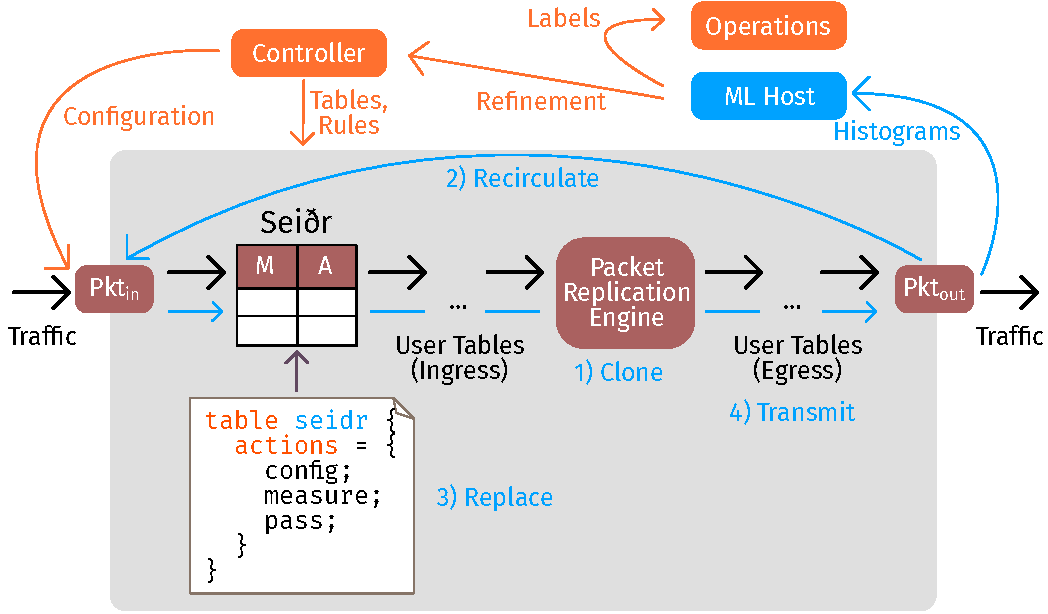
\includegraphics{diagrams/seidr/dp-arch-diagram.pdf}}
    \caption[\seidr{}'s integration with a PSA-compatible dataplane.]{\seidr{}'s integration with a \gls{acr:psa}-compatible dataplane, without the use of digest \texttt{extern}s. \seidr{} uses a register block to store many histograms, each comprised of a fixed bucket count. The main \seidr{} table is used to select which flows or packets are tracked and used in the histogram process, allowing runtime control over monitoring via the control plane. When not using digests to emit telemetry (i.e., for transmission over the control plane), we must rewrite and modify cloned packets to contain the histograms---shown in blue.}
    \label{fig:arch}
\end{figure}

% Let's show them a histogram datastructure would look like purely with registers and how would a P4 action populate it - pseudocode or P4 snippet would be nice.
%\sidenote{?? FIGURE::: Can I redo this diagram to show the possibility of digest?}
Although packet timing information is useful in understanding network and flow behaviour, without volume or packet rate reduction it's prohibitively expensive for hosts to handle each packet.
Histogramming acts as the \emph{aggregation step} which makes this class of analysis feasible in high-speed networks.
\Cref{fig:arch} demonstrates how \seidr{}, installed as an additional table in any P4 program, records and transmits inter-arrival time histograms.
The format for these histogram packets is outlined in \cref{fig:seidr-headers}; bucket counts and size are fixed at compile time.
I choose here to store individual buckets as \mintinline{rust}{u16}s, and fix the number of buckets to \num{100} per histogram as an example (and in later evaluation).
Packets traverse a table which requires \num{3} actions to be implemented:
\begin{enumerate}
    \item \texttt{config} reads any matched packets as a \texttt{seidr\_cfg\_t} of type \texttt{SET\_}\{ \texttt{MIN}, \texttt{MAX}, \texttt{DST}, \texttt{SRC}, \texttt{LEN} \} by using the P4 parser.
    These update registers \numrange{1}{5} in \cref{tab:registers}, dropping any matched packets.
    
    \item \texttt{measure} calculates the inter-arrival time, update per-flow histograms, and transmits finished histograms to the correct host. I describe its operation in \cref{alg:measure}.
    
    \item \texttt{pass} ignores packets, and is the default action.
\end{enumerate}
Constructing \seidr{} in this manner allows the control plane to install rules to enable or disable runtime reconfiguration as needed, and to monitor as many or as few flows as desired (\ie, using wildcard rules or exact matching).

\begin{figure}
\centering
\begin{subfigure}{0.45\linewidth}
\centering
\adjustbox{max width =\linewidth}{
\begin{minipage}{\linewidth}
\begin{minted}[escapeinside=||]{rust}
|\textbf{\textcolor{Keyword}{header}}| seidr_cfg_t {
    bit<8> function;
    bit<144> payload;
}
\end{minted}
\end{minipage}
}
\end{subfigure}
\begin{subfigure}{0.45\linewidth}
\centering
\adjustbox{max width =\linewidth}{
\begin{minipage}{\linewidth}
\begin{minted}[escapeinside=||]{rust}
|\textbf{\textcolor{Keyword}{header}}| seidr_t {
    bit<128> src_ip;
    bit<128> dst_ip;
    bit<16> src_port;
    bit<16> dst_port;
    bit<16> eth_type;
    bit<BUCKETS * 16> histo;
}
\end{minted}
\end{minipage}
}
\end{subfigure}
\caption{P4 headers for \seidr{} configuration and histograms.}\label{fig:seidr-headers}
\end{figure}

\begin{algorithm}
% \vspace{-0.25cm}
% \DontPrintSemicolon
\KwData{5-tuple, P4 metadata, P4 headers, Registers}
h $\leftarrow$ hash(5-tuple)\label{algline:prep-start}\;
index $\leftarrow$ BUCKETS * h\;
owner $\leftarrow$ HistoOwner[h]\label{algline:prep-end}\;
\uIf{metadata.packet\_path = RECIRCULATE}{
    headers.tcp.valid $\leftarrow$ false\label{algline:rewrite-start}\;
    headers.udp.valid $\leftarrow$ true\;
    headers.seidr.valid $\leftarrow$ true\;
    copy 5-tuple into headers.seidr\;
    rewrite headers.ip, headers.udp using HistoSrc/Dest\;
    headers.seidr.histo $\leftarrow$ HistoData[index..]\;
    truncate payload\;
    zero out registers: BucketCount, HistoOwner[h], HistoData[index..]\;\label{algline:rewrite-end}
}
\ElseIf{owner = 0 \textbf{or} owner = 5-tuple}{\label{algline:owner-check}
    HistoOwner[h] $\leftarrow$ 5-tuple\label{algline:iat-prep-start}\;
    iat $\leftarrow$ LastTimestamp[h] - metadata.mac\_ingress\_time\label{algline:iat-prep-end}\;
    \If{iat $\ge$ Min \textbf{and} iat $\le$ Max}{
        bucket $\leftarrow$ BUCKETS * (iat - Min) / (Max - Min)\label{algline:bucket-start}\;
        HistoData[index + bucket] $\leftarrow$ HistoData[index + bucket] + 1\;
        BucketCount[h] $\leftarrow$ BucketCount[h] + 1\label{algline:bucket-end}\;
        \If{BucketCount[h] = Len\label{algline:emitcheck}}{
            mark packet for cloning and recirculation\label{algline:recirc}\;
        }
    }
	LastTimestamp[h] $\leftarrow$ metadata.mac\_ingress\_time\label{algline:update-ts}\;
}

\caption{\seidr{} histogram update and transmission.}\label{alg:measure}
\end{algorithm}

\seidr{}'s operation---\cref{alg:measure}---is generally rather simple.
For now, we will leave aside \crefrange{algline:rewrite-start}{algline:rewrite-end} until \cref{sec:seidr-histo-tx}.
When a flow is to be measured, we first hash its 5-tuple ($h$) and determine which flow is currently occupying slot $h$ (\crefrange{algline:prep-start}{algline:prep-end}).
In the event of hash collision (\cref{algline:owner-check}), we ignore packets outside of the tracked flow to ensure that data is accurate.
As later processing and classification directly affect what decisions are made by operators or automatically taken by a policy (possibly leading to incorrect flow limits, QoS, \emph{etc.}), avoiding corruption/cross-contamination of operational data is paramount.
If the slot is unoccupied or belongs to the current flow, we compute the \gls{acr:iat} and assert ownership over the hash table slot (\crefrange{algline:iat-prep-start}{algline:iat-prep-end}).
Assuming the computed \gls{acr:iat} is within bounds, we compute its bucket index in this interval and increment that bucket and a global counter (\crefrange{algline:bucket-start}{algline:bucket-end})---the global counter triggers a packet emission if it exceeds a known \emph{Len} (\cref{algline:emitcheck}).
Finally, we update the flow's last timestamp (\cref{algline:update-ts}).
To gain collision resistance, \emph{Robin Hood}~\parencite{DBLP:conf/focs/CelisLM85} or \emph{Cuckoo}~\parencite{DBLP:conf/esa/PaghR01} hashing could be used up to a maximum distance in the table, treating a zeroed owner as empty and an illegal source \gls{acr:ip} address as a tombstone value.

\begin{table}
    \centering
    \caption{\seidr{} register map and required sizes using an an $h$-bit hash.}
%    \resizebox{\linewidth}{!}{
    	\expandableinput{tables/seidr/registers}
%    }
    \label{tab:registers}
\end{table}

% Basic Logic:
% \begin{itemize}
%     \item table 1: three actions
%     \begin{itemize}
%         \item config: set R1 or R2 (controller installs rule matching a specific port/ip combo)
%         \item measure: take ingress timestamp from metadata, do stuff, write into lasttime, add to bucket and total if within bounds
%         \item pass (default)
%     \end{itemize}
%     \item then pass onto rest of tables
%     \item Why do it this way? can make it all or nothing through control plane.
%     \item How to write and send packet? Same trick as ESNET? (recirc w/ custom metadata to transform pkt)
% \end{itemize}

% ?? NOTE: See PSA \cite{p4-psa} for register format. Some papers, like Dapper, suggest that hash tables should be possible? That would work out very well in our benefit.

% ?? What is configurable? Min, max of the histogramming range

This design allows runtime configuration of all aspects save for the bucket count; at runtime, the only way to increase bucket resolution is to examine a smaller region of \glspl{acr:iat}.
While in theory this could be configured below a maximum compiled into the firmware, the difficulties introduced by classification and later data processing make this infeasible.
Unless using stream-capable classifiers such as \glspl{acr:lstm}, changing the input size requires retraining from scratch since new neuron weights must be added and structural properties of the input data change.
Increasing the bucket count requires new firmware installation, as many dataplane P4 implementations cannot allocate variable-length stores due to the lack of a dynamic allocator.

\begin{figure}[]
    \centering
    \begin{subfigure}[t]{\linewidth}
        \centering
        \resizebox{\linewidth}{!}{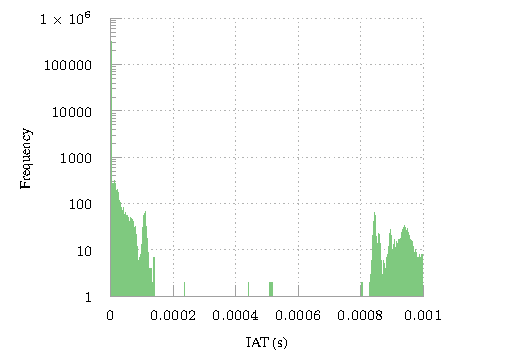
\includegraphics{plots/seidr/dt-cubic-1000-app.pdf}}
        \subcaption{TCP Cubic}
        \label{fig:cubic-hist-app}
    \end{subfigure}

    \begin{subfigure}[t]{\linewidth}
        \centering
        \resizebox{\linewidth}{!}{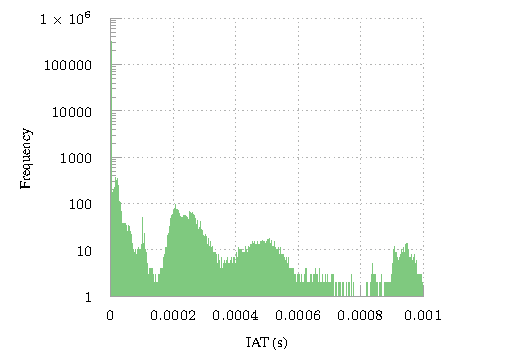
\includegraphics{plots/seidr/dt-bbr-1000-app.pdf}}
        \subcaption{TCP BBR}
        \label{fig:bbr-hist-app}
    \end{subfigure}

    \caption[Example dataplane histograms showing visible differences in inter-arrival times of selected TCP flavours.]{Example dataplane histograms showing visible differences in inter-arrival times of selected \gls{acr:tcp} flavours. These plots examine sub-\qty{1}{\milli\second} dynamics of two separate flows of \qty{1000}{\mega\bit\per\second} traffic generated according to \cref{sec:seidr-datasets}, over these flows' entire lifecycles. BBR flows have significantly more \glspl{acr:iat} measured in the \qtyrange{100}{800}{\micro\second} band, with additional structural differences outside this significant region.}
    \label{fig:tcp-hist-app}
\end{figure}

As a visual example of dataplane-generated histograms, \cref{fig:tcp-hist-app} shows the distribution of inter-arrival times between two \gls{acr:tcp} congestion control algorithms under otherwise identical conditions.
While I cover the underlying causes for these stark differences in more detail later (\cref{sec:seidr-tcpcc}), it should be clear that there are variations in the \emph{distribution} of features that are visible to us (as humans) quite plainly.
It stands to reasons that they should also be visible to a trained \gls{acr:ml} classifier.
%The visible differences are programmatically identified later in \cref{sec:seidr-evaluation} using our \gls{acr:ml} algorithms.
While these particular histograms are taken at the macro level---over the entire lifecycle of a flow---this also gives us cause to look into shorter measured windows.

\subsection{Histogram transmission}\label{sec:seidr-histo-tx}
When targeting the P4-\gls{acr:psa}, we have some options in how histograms may be transmitted from the \gls{acr:pdp} hardware of interest---either to the control plane or dataplane.
If we choose to emit histogram packets to the control plane, we may make use of \emph{digest} \texttt{extern}s which are offered by many \gls{acr:psa}-compliant devices (though aren't strictly required).
Practically speaking, these allow us to pack and emit arbitrary \texttt{struct}s which are delivered to the attached controller \gls{acr:cpu} over the P4Runtime \gls{acr:api}.

\Cref{alg:measure,fig:arch} instead show a more complex case, where we emit generated histogram packets in-band on the dataplane.
The \gls{acr:psa} does not have any explicit mechanisms for generating new packets to be carried by the \emph{dataplane}.
To circumvent this, any packet which would complete a histogram is tagged for cloning at the end of the ingress pipeline, and recirculation at egress (\cref{algline:recirc}).
This truncated copy returns to \seidr{}'s table, where we enable the relevant headers, change L2/3 fields, and write out the histogram contents (\crefrange{algline:rewrite-start}{algline:rewrite-end}).
The P4 deparser outputs the new protocol stack at egress, and transmits the histogram UDP packet into the network.
Although achieved in a somewhat roundabout way, this does have an upside in that it's compatible with the guaranteed core functions of the \gls{acr:psa}.
In future, event-driven architecture proposals~\parencite{DBLP:conf/hotnets/IbanezABM19} may allow first-class support for packet generation.

There are tangible reasons to prefer emitting histograms to the dataplane in spite of the added complexity and recirculations.
Although the data volume and packet-per-second reductions offered by \seidr{} histograms are strong, the former case pushes the steering of all generated packets onto a single controller per switch.
Intuitively, this is expensive and may very well interfere with regular operation of the control plane.
On the other hand, outputting histograms over the dataplane allows administrators to make use of existing \glspl{acr:asic}-backed infrastructure to load-balance classifications across typical host machines.
Alternatively, we might forward packets directly to dedicated, network-connected accelerators like BrainWave whose outputs then inform control plane operation.
Both of these cases spare the control plane of extra load, at modest additional bandwidth cost due to the reduction in telemetry volume.
Digests of course have their own benefits: in some \gls{acr:psa} implementations they may be built in the egress pipeline, adding flexibility for how \seidr{} might be integrated with existing forwarding plane designs (rather than forcing its inclusion in the \emph{ingress} pipeline).

%?? outline benefits and drawbacks of each.
%
%?? talk abt new stuff in heres.
%
%?? Big open qs:
%?? relevance of PSA digests? These can emit packets, no? These can emit an arbitrary struct to the ctl plane over P4Runtime API. Might be good if no digest support, . Digests have a few extra benefits: In some dataplanes can be emitted in egress. Is message fusion a possible downside? (unpredictable)
%?? Maybe 2 options? Can be in-band or out-of-band. Digests are the out-of-band option, meanwhile in-band allows you to use dataplane to forward to accelerators like BrainWave (don't add extra load to ctl plane in this way?)

%?? Header size limits are the other main constraint.
%?? THis is probably not a problem with digests.
%?? WHen emitting to dataplane, however? Will have plat-dependent limits on output. Header size limits, PHV limits, register access reqs that could prevent digest access? Need to mark in-progress histo emissions, progress for each, and emit bitslices spread over multiple egress pkts. Logic: CLONE LOOP WHile still pkts to write, block updates to histo if progress (1 bit?). Limitation: Histo emission freq must be reduced to prevent massive traffic amp. slicing logic could be extended to include the digest case? Are there PHV limits in the digest case that make this really suck?

Another design constraint where these two differ is in header-size limits\sidenote{These designs and implementations again focus on using Netronome \gls{acr:nfp} SmartNICs, as opposed to Tofino \gls{acr:rmt} hardware where such limits do in fact apply.}.
In the case of digests we can assume that a P4 switch is capable of emitting larger packets: following the specification, switches are free to collate generated digests together before handing them off to the control plane.
For transit via the dataplane, however, platform-dependent limits will apply to output packets---particularly as we must use rewritten header fields for this purpose.
This leads to a problem which \cref{alg:measure} does not directly account for: histogram data may be larger than headers allow for.
To fix this, we must make some high-level modifications to its behaviour.
We must mark in-progress transmissions and emit bitslices from the output histogram split over several egress packets by performing a clone loop, where each non-terminal histogram packet is cloned and marches the `send window' forward.
Until termination, updates to the histogram's recorded data are blocked.
A key limitation, however, is that the histogram generation frequency and other parameters must be tuned to prevent traffic amplification driven by the switch.

\subsection{Accurate, precise and high-resolution timestamping}

Precise timestamps are critical when detecting temporal properties of flow behaviour, such as microbursts or inferring flow congestion control algorithms.
It is especially important in high speed (\qty{100}{\giga\bit\per\second}) networks, where there can be as little as \qty{6.7}{\nano\second} between packets that need to be analysed.
With a Linux-based software solution (\eg, reading packets from a link with \emph{tcpdump}), the Linux kernel can only provide microsecond-level accuracy with precision in the order of \qty{100}{\micro\second}~\parencite{DBLP:conf/noms/KundelSBRK20}.
\gls{acr:dpdk} improves on this, increasing the accuracy to \qty{100}{\nano\second} in the best case~\parencite{DBLP:journals/ccr/PrimoracBA17}.
However, today's dataplane devices (\eg, Netronome SmartNICs, NetFPGA SUME) allow nanosecond-accurate timestamps to be retrieved from the \gls{acr:mac} modules with a precision of \qty{10}{\nano\second}~\parencite{DBLP:conf/noms/KundelSBRK20}, a timestamp property \seidr{} relies upon.

% Some platforms provide picosecond-level precision and many solutions allow time synchronisation between multiple devices using the IEEE 1588-2002 (Precision Time Protocol) standard.



\section{TCP congestion control classification}\label{sec:seidr-tcpcc}


% We present an example of first-stage analysis performed for each flow and each packet---stateful TCP analysis.
% This includes numerous metrics which are considered standard when measured at connection endpoints, yet are difficult or invite numerous issues when performed in the network (of which we include a discussion on drawbacks and, curiously, benefits).
% The introduction of accurate timestamps allows us to explore rate-monitoring at a per-packet level, a new view of flow behaviour which may enable flow and hardware characterisation.

% \subsection{Per-Packet Rate Monitoring}

% \begin{figure*}
%     \centering
%     \begin{subfigure}[t]{0.49\linewidth}
%         \centering
%         \resizebox{0.5\linewidth}{!}{
% 	    \begin{tikzpicture}
%     		[packet/.style={draw, fill=uofgsunshine}]
% 		    \node[packet] (p1) {$p_1$: 1500B};
% 		    \node[packet, right= 1cm of p1] (p2) {$p_2$: 800B};
		
% 		    \node at ($(p1.south west) - (0,1)$) (t1) {$t_1$};
% 		    \node at ($(p2.south west) - (0,1)$) (t2) {$t_2$};
		
% 		    \draw[-, dotted] (t1.north)--(p1.south west);
% 		    \draw[-, dotted] (t2.north)--(p2.south west);
		
%     		\draw[<->] (t1.north) -- node[below]{$\mathit{dt}$} (t2.north);
% 	    	\draw[<->] ($(t1.north) + (0,0.2)$) -- node[above]{$s$} ($(t1.north) + (1.8,0.2)$);
% 		    \draw[<->] ($(t1.north) + (1.8,0.2)$) -- node[above]{$g$} ($(t2.north) + (0,0.2)$);
% 	    \end{tikzpicture} 
% 	}
%     \caption{\centering Per-packet rate, visualised. Note that $p_1$ and $p_2$ are not necessarily packets from the same flow.}
%     \label{fig:per-packet-rate}
%     \end{subfigure}
%     \begin{subfigure}[t]{0.49\linewidth}
%     \centering
%     \resizebox{0.9\linewidth}{!}{
% 		\begin{tikzpicture}
% 		[packet/.style={draw, fill=uofgsunshine}]
% 		\node[packet] (p1) {$p_1$: 1500B};
% 		\node[packet, right= 1cm of p1] (p2) {$p_2$: 800B};
% 		\node[right= 1cm of p2] (p3) {...};
% 		\node[packet, right= 1cm of p3] (p4) {$p_{n-1}$: 1500B};
% 		\node[packet, right= 1cm of p4] (p5) {$p_n$: 1500B};
		
% 		\node at ($(p1.south west) - (0,1)$) (t1) {$t_1$};
% 		\node at ($(p2.south west) - (0,1)$) (t2) {$t_2$};
% 		\node at ($(p4.south west) - (0,1)$) (t4) {$t_{n-1}$};
% 		\node at ($(p5.south west) - (0,1)$) (t5) {$t_{n}$};
		
% 		\draw[-, dotted] (t1.north)--(p1.south west);
% 		\draw[-, dotted] (t2.north)--(p2.south west);
% 		\draw[-, dotted] (t4.north)--(p4.south west);
% 		\draw[-, dotted] (t5.north)--(p5.south west);

%         \draw[<->] ($(t2.south) + (0,-0.25)$) -- node[above]{$s$} ($(t2.south) + (6.25,-0.25)$);
%         \draw[<->] ($(t2.south) + (6.25,-0.25)$) -- node[above]{$g$} ($(t5.south) + (0,-0.25)$);
% 		\draw[-, thick] ($(t2.south) - (0,0.5)$) -- node[below]{$W$} ($(t5.south) - (0,0.5)$);
% 		\end{tikzpicture} 
% 	}
%     \caption{\centering Sliding window rate, visualised. Rate estimates are computed using the sizes of the last $W$ packets seen in the current flow. Packets $p_2$ and $p_{n-1}$ belong to the same flow, but $p_n$ is not assumed to.}
%     \label{fig:sliding-window-rate}
%     \end{subfigure}
%     \caption{Comparison of per-packet and sliding window rates. The lengths of packets and inter-packet gaps are not to scale, and are purely demonstrative.}
%     \label{fig:pr-vs-slide}
% \end{figure*}

% Associating each packet with a high-resolution timestamp allows us to introduce the notion of a \emph{per-packet rate}.
% Assuming a packet with size $p$ arrives at time $t_1$ and is followed by another packet (potentially from another flow) which arrives at $t_2$, we measure $\mathit{dt}=t_2-t_1$ for this packet.
% Supposing this first packet spends time $s$ on the wire and assuming that the inter-packet gap $g$ is negligible compared to the length of a packet, then $\mathit{s} = \mathit{dt} - g \approx \mathit{dt}$.
% This packet then has a point rate, $r$:
% \begin{equation}
%     r = \frac{p}{s} \approx \frac{p}{\mathit{dt}}
% \end{equation}
% \Cref{fig:pr-vs-slide} demonstrates how this timing information arises, contrasted with sliding-window rate measurements taken over a longer time period.
% This assumes almost back-to-back traffic, which is realistic in our deployment environment, but to the best of our knowledge no programmable switches expose the timestamp at which the final bit of a packet has been ingested.
% Such a timestamp would allow exact measurement of $s$.

% % ?? we need to be clear about the unintuitive nature of these measurements, include a quick sketch proof which shows that the weighted average of a set of point rates is analytically identical to the sliding window rate/throughput taken over the same period of time.
% While this is an interesting measure to associate with each packet, considering how best to view such rates in aggregate can be counter-intuitive.
% Viewing these rates as time series data reveals interesting distributional characteristics which disagree starkly with our understanding of a flow's rate---for instance, clusters which suggest a different mean.
% Suppose we have a set of measurement indices $C$ with no gaps captured between $t$ and $t'$, partitioned into flows $C = F_1 \cup \dots \cup F_p$.
% To correctly combine a set of point measurements for a flow $F_i$ into an average rate $\overline{r}_{F_i}$, we compute:
% \begin{equation}
%     \overline{r}_{F_i} = \frac{\sum_{a \in F_i} \mathit{dt}_a r_a}{\sum_{c \in C} \mathit{dt}_c}.
% \end{equation}
% In the instance that only one flow is captured (\emph{i.e.}, $F_i = C$), this is a weighted average over point rates, using the $\mathit{dt}$ measured between each packet and the next packet in the same flow as its weight.
% Similarly, this is analytically equivalent to the sliding-window rate measured over the same set of packets:
% \begin{equation}
%     \frac{\sum_{a \in F_i} \mathit{dt}_a r_a}{\sum_{a \in F_i} \mathit{dt}_a} \simeq \frac{\sum_{a \in F_i} p_a}{t' - t}.
% \end{equation}
% % \begin{proof}
% % Given a set of contiguous measurements from the same flow $S \subseteq \mathbb{Z}$, admitting $p_s$, $r_s$, $\mathit{IAT}_s$ and $t_s$, the weighted average of point rates is then
% % $$
% % \overline{r}_S = \frac{\sum_{s \in S} \mathit{IAT}_s r_s}{\sum_{s \in S} \mathit{IAT}_s}
% % $$
% % The sliding-window average:
% % $$
% % \overline{r}_S = \frac{\sum_{s \in S} \mathit{IAT}_s r_s}{\sum_{s \in S} \mathit{IAT}_s}
% % $$
% % \end{proof}

% We assume that inter-packet gaps will be negligible (\emph{i.e.}, that the link is never in a state of very low utilisation), due to typically high utilisation on a WAN.
% % Similarly, we need to discuss the effects of selective monitoring or an abundance of UDP/ICMP traffic (which will distort $dt$s).
% However, this assumption can be distorted if selective TCP flow monitoring is used, or if UDP/ICMP traffic is overabundant; both these scenarios create larger gaps between TCP packets of interest, inflating $g$ to the point where it is comparable in size to $s$.
% This has an impact on our notion of per-packet rates, but not inter-arrival times or other such dependent metrics.
% The effect is small on sliding window rates, particularly at larger window sizes.
% ?? Justify. On paper, it looked like error term was O(1/n), O(g) for an n packet window.


% \section{Inter-Arrival Time}

% Having assigned each packet in a flow with a nanosecond-accurate timestamp ?? tbc

\Cref{fig:tcp-hist-app} suggests that a notable use-case for this type of measurement is detecting \gls{acr:tcp} flows' choice of \gls{acr:cca}.
In a \gls{acr:tcp} connection, each machine is free to choose the \gls{acr:cca} it uses to send bytes, and thus how it responds to network congestion signals.
This choice is entirely local, and so is invisible to both the other machine and the network.
In data centre networks, operators choose these ahead of time to ensure optimal behaviour, where the environment makes it easy to consistently deploy this choice across all nodes.
This is not the case in most \glspl{acr:as}; in a transit network or large \gls{acr:wan}, these hosts (and thus the \glspl{acr:cca} in use) are outside the control of network operators, which introduces difficulties when \gls{acr:cca} interactions lead to \emph{unfairness}.
Consider the recent (and widespread) introduction of \emph{\gls{acr:tcp} BBR}~\parencite{DBLP:journals/queue/CardwellCGYJ16}.
\emph{BBR} is a delay/model-based \gls{acr:cca} which converges on a fair share of bottleneck bandwidth by reducing its rate if the round-trip time increases, while periodically attempting to increase send rate to account for path or load changes.
However, \emph{BBR} traffic can consume \qty{40}{\percent} of link capacity when multiplexed with loss-based \glspl{acr:cca}, regardless of the number of competing flows~\parencite{DBLP:conf/imc/WareMSS19}. 
When ensuring fair transit to all flows, this is hardly a desirable outcome; in fact, it's one which may frustrate clients or violate \glspl{acr:sla}.

A curious property of \emph{BBR}'s algorithm which sets it apart from other variants is that packet transmission is \emph{timer-based}.
\texttt{send(packet)}, as defined in the canonical algorithm, asks that on transmission of a packet, the sender should wait for the estimated time that packet would take to reach the recipient.
For instance, at an estimated bottleneck bandwidth of \qty{8}{\mega\bit\per\second}, a \qty{1024}{\kilo\byte} packet would hold back the next packet in the flow until \qty{976.6}{\micro\second} had elapsed.
When packet sizes remain similar this causes strongly periodic behaviour, while mode switches in the \emph{BBR} algorithm cause these periodic bands to shift up or down accordingly.
This effect is stronger than in existing loss- and delay-based algorithms which remain intrinsically tied to the notion of a congestion window (where release of buffered packets follows the receipt of \texttt{ACK} messages).
As a result, timing behaviour of past \glspl{acr:cca} may be influenced by (the lack of) packet pacing, periodic components might be made noisier by jitter along the return path, or the behaviour of the receiver might add further noise.

This high-level analysis of \emph{BBR} gives us a strong feature to use as the basis for classification: the \glspl{acr:iat} for each packet in a flow.
We have two options for processing this for classification: we may use a compressed, fixed-size representation such as histograms to capture the aggregate distribution, or we may attempt to capture structural behaviour by using a variable-length stream of \glspl{acr:iat}.
In many networks, the data and packet rate reduction offered by the former is required to make this possible.
Indeed, as we've examined in greater detail through \cref{sec:inc-uses-pdp-ml}, in-switch aggregation has seen great success in aiding \gls{acr:ml} for training~\parencite{DBLP:conf/isca/LiLYCSH19}.
We make use of the following standard classification algorithms on a fixed-size representation to attempt to single out the \gls{acr:cca} in use:

\begin{itemize}
    \item \glsxtrfull{acr:knn}. A simple and well-understood classifier which assigns labels based on the closest members of the training corpus (\ie, by the $\ell_2$ metric). They have a linear runtime memory cost in amount of training data, and no training cost other than loading all data points. However, they are surprisingly capable of learning complex decision boundaries on fixed-length inputs.
    
    \item \glsxtrfullpl{acr:cnn}. As discussed in \cref{sec:ddnlit-nns}, \glspl{acr:cnn} are a neural network approach which learns convolution kernels to classify fixed-length data, particularly when recognising spatial features. Runtime memory cost is fixed for a given architecture irrespective of the amount of training data used, with a high training cost in memory and computation time.
\end{itemize}
% \fakepara{Long Short-Term Memory~\parencite{DBLP:journals/neco/HochreiterS97} units (LSTMs)} A class of recurrent neural network used for stream classification, forecasting, and prediction of variable-length data. Memory cost is fixed, with longer training times (and more data required) than similarly sized CNNs.
% Of these, we apply $k$-NN and CNNs to histograms of packet IATs, and LSTMS to raw IAT streams.

When examining \gls{acr:knn} classifiers, I measured accuracy across choices of $k \in \left[2, 8\right]$; I found $k=2$ to be the most effective choice with these input data using the $\ell_2$ metric.
Our \gls{acr:cnn} architecture is described in \cref{tab:cnn-arch}, using ReLu activation and $1 \times 1$ stride in convolutional layers unless stated otherwise.
Training occurred over 5 epochs using the Adam optimiser with categorical cross-entropy as a loss metric, and a batch size of \num{64} histograms (\num{8} for full sequences due to the smaller data volume).
For \emph{BBR vs.\ Cubic}, the complete model consists of \qtyproduct{104898 x 32}{\bit} floating-point parameters (\qty{409.76}{\kibi\byte}), while the full classification task adds a further \num{130} parameters (\qty{0.51}{\kibi\byte}).

\begin{table}
    \centering
    \caption[CNN architecture for \num{100}-entry histograms.]{\gls{acr:cnn} architecture for \num{100}-entry histograms.}
%    \resizebox{0.7\linewidth}{!}{
    	\begin{tabular}{cccc}\toprule
        Layer & Nodes/Filters & Filter Size & Output Dimension \\ \midrule
        Conv2D & 32 & \numproduct{3 x 1} & \numproduct{98 x 1 x 32} \\
        MaxPool & --- & \numproduct{2 x 1} & \numproduct{49 x 1 x 32} \\
        Conv2D & 64 & \numproduct{3 x 1} & \numproduct{47 x 1 x 64} \\
        MaxPool & --- & \numproduct{2 x 1} & \numproduct{23 x 1 x 64} \\
        Conv2D & 64 & \numproduct{3 x 1} & \numproduct{21 x 1 x 64} \\
        Flatten & --- & --- & \num{1344} \\
        Dense & 64 & --- & \num{64} \\
        Dense (Softmax) & $n_\mathit{classes}$ & --- & $n_\mathit{classes}$ \\
        \bottomrule
    \end{tabular}
%}
    \label{tab:cnn-arch}
\end{table}


\section{Evaluation}\label{sec:seidr-evaluation}
%Traffic is played back from hosts via Tcpreplay at a bandwidth assigned uniformly from a `good' or `bad' distribution, each using the same pcap file with source and destination IP addresses rewritten.

This work is most naturally compared against Marl, introduced by \textcite{DBLP:journals/eaai/MalialisK15}, the state-of-the-art in \gls{acr:rl}-based \gls{acr:ddos} prevention.
We are most interested in seeing how their approach contrasts with the new agent designs across different topologies and workloads.
Different network environments will also impose different levels of host density, where popular web servers may have orders of magnitude more clients than egress points from their network---I aim to show how these characteristics affect performance and learning rate.
Marl is known to outperform the AIMD~\parencite{DBLP:journals/ton/YauLLY05} strategy, yet the state of the art has long since moved on.
To paint a more current picture, I compare this work against an effective modern approach, \emph{SPIFFY}~\parencite{DBLP:conf/ndss/KangGS16}.
SPIFFY tests a proportion of flows by routing them through an alternate path with higher bandwidth, observing how their speed changes some time later.
This comparison lets us position our new agent designs against the state of the art, observing that SPIFFY has a similar mode of interaction to \gls{acr:rl}-based systems (taking action, observing an effect, and acting once again) and does not rely on protocol characteristics or signatures.
In reimplementing SPIFFY, I make the simplifying assumption that a suitable unused path exists (with identical bandwidth to the server's link).
\qty{10}{\percent} of active flows were tested at a time (according to the authors' observation that there is a factor of \qty{10}{\times} difference between the ideal and achieved bandwidth expansion), excluding flows below \qty{50}{\kilo\bit\per\second} and requiring a \qty{3}{\times} expansion from legitimate flows, making a judgement after \qty{5}{\second}.

To test this, I made use of both traffic models introduced in \cref{sec:a-new-normal} (Opus and \gls{acr:tcp}), both topologies discussed below (1-dest vs.\ Fat-Tree), and vary the amount of hosts typically communicating over each agent's ingress/egress node.
Additionally, these new models were evaluated in multi-agent mode (\emph{separate}, no model sharing), and in single-agent mode (\emph{single}, zero-cost perfect information sharing).
In each case, the algorithm's performance was averaged over \num{10} episodes of length \num{10000} timesteps (setting each agent's $\wvec{}=\mathbf{0}$ between episodes).
Host allocations at the beginning of each episode were generated pseudorandomly to ensure fairness between episodes---a host is malicious with probability $\operatorname{P}\left(\mathit{malicious}\right)$, and is benign otherwise.
Benign hosts generate traffic according to either \cref{sec:tcp-http-traffic-model,sec:udp-opus-traffic-model} depending on the experiment, while malicious hosts generate traffic as described in \cref{sec:attack-traffic-model} (both at experiment-dependent rates).

All experiments were executed on Ubuntu 18.04.2 LTS (GNU/Linux 4.4.3-040403-generic x86\_64), using an Intel Core i7-6700K (\qtyproduct[product-units=single]{4 x 4.2}{\giga\hertz}) which had \SI{32}{\gibi\byte} of \gls{acr:ram}.
%All code underpinning these findings is available on a public repository\footnote{\url{https://github.com/FelixMcFelix/rln-dc-ddos-paper}}.
%All code underpinning these findings is available on a public repository.\footnote{Private until publication.}

\subsection{Single destination}\label{sec:single-dest}
%?? Move description of tree topol to here.
The network is tree-structured, where one server $s$ connects through a dedicated switch to $k$ team leader switches, each connected to $\ell$ intermediate switches, which in turn each connect to $m$ egress switches.
We then have $N_{\mathit{hosts}} = k \ell m n$.
\Cref{fig:marl-topol} demonstrates this.
%Although \citeauthor{DBLP:journals/ccr/MahajanBFIPS02a}, the originators of this topology, make it clear that it exists as a fairly unrepresentative example \cite{DBLP:journals/ccr/MahajanBFIPS02a}, it remains the case that such a network topology allows for functional testing, and indeed is illustrative of one way in which attack traffic might aggregate in the network.
%It is hard, however, to argue its relevance to specific classes of victim or to reason about the interactions it might have with dependent applications.
%We aim to address this through \cref{sec:performance-in-an-emulated-environment}.
The network topology was configured using $k=2$ teams, $\ell=3$ intermediate nodes per team, $m=2$ agents per intermediate node, and $n \in \{2, 4, 8, 16\}$ hosts per learner.
This is a slight simplification of \Textcite{DBLP:journals/eaai/MalialisK15}'s \textquote{online} experiment, choosing fewer teams but remaining as a single server with a fan-out network.
%The algorithm parameters were set at $\gamma=0$ (leading to opportunistic behaviour), $\alpha=0.05$, having linearly annealed $\epsilon=0.2 \rightarrow 0$ by $t=3000$.
%Benign and malicious hosts uploaded between \SIrange{0}{1}{\mega\bit\per\second} and \SIrange{2.5}{6}{\mega\bit\per\second} respectively, and hosts were redrawn at each episode's start with $\operatorname{P}(\mathit{malicious})=0.4$.
%$U_s$  $k \ell mn+2$ \si{\mega\bit\per\second}.
%The performance of each choice of $n$ was averaged over \num{10} episodes of length \num{10000} timesteps (setting each agent's $\wvec{}=\bm{0}$ between episodes).
%Host allocations were generated pseudorandomly to ensure fairness between choices of $n$.
%These parameter choices match those of the original study to enable direct comparison, and are (to the best of our knowledge) arbitrary, but we justify our range of $n$ as capturing increasing scales of host activity.

\begin{figure}
	\centering
	\resizebox{0.9\linewidth}{!}{\begin{tikzpicture}[
	texts/.style = {text=black},
	labeltexts/.style = {text=uofgsandstone},
	treeline/.style = {draw=uofgburgundy},
	treenode/.style = {texts, circle, centered, fill=white, treeline},
	load/.style = {fill=uofgcobalt},
	loadhide/.style = {fill=uofgcobalt!40!white},
	external/.style = {fill=uofgrust},
	externalhide/.style = {fill=uofgrust!40!white},
	hideline/.style = {draw=uofgsandstone!40!white},
	hidenode/.style = {treenode, hideline},
	grow'=right
]
	\node[treenode, label={[texts]above:Server}] (root) {}
	child [treeline] { node [treenode, label={[texts]above:Core}] (sswitch) {}
		child [treeline] { node [treenode, label={[texts]above:Leader}] (teaml) {} 
			child [treeline] { node [treenode, label={[texts]above:Intermediate}] (inter) {}
				child [treeline] { node [treenode, load, label={[texts]above:Agent/Egress}] (agent) {}
					child [treeline] { node [treenode, external] (extern) {}
						child [treeline] { node [treenode, external, label={[texts]above:Host}] (host) {} }
						child [hideline] { node [hidenode, externalhide] (endhost) {} }
					}
				}
				child [hideline] { node [hidenode, loadhide] (endagent) {} }
			}
			child [hideline] { node [hidenode] (endinter) {} }
		}
		child [hideline] { node [hidenode] (endteaml) {} }
		edge from parent
		node[below, labeltexts] {$U_s$}
	};
	
	%\draw[-] (teaml) -- (endteaml);
	\node [labeltexts] (kdots) at ($(teaml)!0.5!(endteaml)$) {$\rvdots$};
	\node [labeltexts, right = -0.1cm of kdots] {$k$};
	\node [labeltexts] (ldots) at ($(inter)!0.5!(endinter)$) {$\rvdots$};
	\node [labeltexts, right = -0.1cm of ldots] {$\ell$};
	\node [labeltexts] (mdots) at ($(agent)!0.5!(endagent)$) {$\rvdots$};
	\node [labeltexts, right = -0.1cm of mdots] {$m$};
	\node [labeltexts] (ndots) at ($(host)!0.5!(endhost)$) {$\rvdots$};
	\node [labeltexts, right = -0.1cm of ndots] {$n$};
\end{tikzpicture}}
	\caption[Tree-structured network topology diagram for evaluating a single-destination network.]{
		Network topology diagram, showing how the server and its core switch's $k$ teams are structured, with $\ell$ intermediate routers per team, connected to $m$ agents which each moderate $n$ hosts beyond a single external switch.
		%	Empty nodes are considered to be internal.
		Red nodes are external, and each blue node hosts an agent.
		\label{fig:marl-topol}
	}
\end{figure}

\subsection{Multiple destinations}
The previous topology allows for direct comparison against the state-of-the-art, and indeed is illustrative of one way in which attack traffic might aggregate in the network.
It is hard, however, to argue its relevance to specific classes of victim or to reason about the interactions it might have with dependent applications.
In contrast, the fat-tree topology~\parencite{DBLP:conf/sigcomm/Al-FaresLV08} sees regular use in real-world data centres and scales well horizontally.
%?? Come up with description of fat-tree (multi-dest) topol.
%?? Why fat tree? regularly appears in modern datacentres.
%?? $k=4$ fat-tree , with one pod hosting two servers $s_0,s_1$.
We use a $k=4$ fat-tree, with one pod hosting two servers $s_0$ and $s_1$.
$n$ external hosts connect through each core switch (where agents are hosted), and communicate with $s_0, s_1$ uniformly randomly.
Both servers host identical services.
We set $n \in \{6, 12, 24, 48\}$ hosts per learner (keeping $N_{\mathit{hosts}}$ identical to each tier of the single-host topology), and restrict $U_{s_0} = U_{s_1} = U_s / 2$.

\subsection{Parameters}
The algorithm parameters were set at $\alpha=$~\num{0.05}, linearly annealing $\epsilon=$ \num{0.2} $\rightarrow$ 0 by $t=$~\num{3000} in the case of Marl (\num{8000} actions per agent in the \emph{Instant/Guarded} models).

Benign hosts each occupied \qtyrange{0}{1}{\mega\bit\per\second}, and hosts were redrawn at each episode's start with $\operatorname{P}(\mathit{malicious})=$~\num{0.4}.
%The original introduction of this approach to direct-control reinforcement learning as introduced by \textcite{DBLP:journals/eaai/MalialisK15} fails to consider key cases: the absence of a suitable heuristic classifier $g(\cdot)$, disjoint ranges of traffic distribution (i.e., the presence of benign heavy-hitters), the accurate simulation of TCP-like behaviour (and its effects on collateral damage), and high densities of hosts at egress points.
%?? Why? ...
%Of these, the latter two are most deserving of a closer investigation, as they have stronger implications for wide-scale deployment.
%These are important issues, particularly when we consider real-world deployment.
%Heuristic estimates of traffic legitimacy come with computational cost and couple the reward function to the accuracy of the estimator, hosts often show diversity in their own traffic patterns (perhaps being multi-modal), and it is known that TCP is the most used transport protocol for Internet traffic \cite{DBLP:conf/saint/ZhangDJC09}.
%?? NEED TO VERIFY VOLUME OF CONGESTION-AWARE PROTOCOLS
Malicious hosts each sent \qtyrange{2.5}{6}{\mega\bit\per\second} when attacking \gls{acr:udp} traffic, though this was increased to \qtyrange{4}{7}{\mega\bit\per\second} when using \gls{acr:tcp}-like traffic (to meaningfully impact benign flows).
Given $n$ and $\operatorname{P}(\mathit{malicious})$, we see an expected malicious bandwidth \numrange{1.27}{1.87} and \qtyrange{2.03}{2.18}{\times} $U_s$ respectively.
%The expected fraction of $U_s$ consumed by each host is \SI{21.5}{\percent} for $n=2$, and \SI{2.84}{\percent} for $n=16$.
For these choices of $n$ in both topologies, we observe $N_{\mathit{hosts}} \in \left\{24, 48, 96, 192\right\}$, and an expected number of malicious hosts $\mathbb{E}\left[N_{\mathit{attackers}}\right] \in \left\{9.6, 19.2, 38.4, 76.8\right\}$.
For the largest choice of $n$, we see an expected total attack traffic $\mathbb{E}\left[V_{\mathit{attack}}\right] =$ \qtylist{334.05;422.4}{\mega\bit\per\second} for Opus and \gls{acr:http} traffic respectively.

$U_s$ was fixed at $N_{\mathit{hosts}}+2$ \unit{\mega\bit\per\second} (to account for burstiness), and each link had a delay of \qty{10}{\milli\second}.
All links had unbounded capacity, save for each server-switch.
These parameters match those of the original study to enable direct comparison, and many are (to the best of our knowledge) arbitrary, but I justify the range of $n$ as capturing increasing scales of host activity.

% \section{Related Work}\label{sec:related}
% %?? Try and compare my work here when possible?

\fakepara{DDoS Prevention}
\Textcite{DBLP:conf/lcn/BragaMP10} examine the detection of flooding DDoS attacks through \emph{self-organising maps}, using SDN to gather statistics effectively.
Many of their features aren't overly relevant, as their focus is not active defence or discovering \emph{which} hosts contribute to an attack.
%?? Actually talk about Marl (???) to appease reviewer \#1.
The closest available approach within this field is that of \textcite{DBLP:journals/eaai/MalialisK15} (whom we have positioned our work against), and their contribution in applying RL to the task of intrusion prevention is significant: their work helps to show the viability of live, adaptive, feedback-loop-like control of the network to detect and prevent DDoS attacks.
They create a tree overlay topology (subdivided into teams), where each agent applies packet drop to \emph{all} flows inbound to a protected server.
%?? Recap their flaws, since they've been cut form every other aspect.
Our results show that their technique underperforms at high host density and when congestion-aware traffic dominates---that their results do not demonstrate this suggests an evaluation driven purely by traces (rather than live application dynamics).

\emph{SPIFFY} \cite{DBLP:conf/ndss/KangGS16} aims to remedy transit-link attacks by observing how flows from each source respond to a sudden increase in available bandwidth.
\Citeauthor{DBLP:conf/ndss/KangGS16} realise that bots participating in an attack are often unable to match this bandwidth expansion (having already saturated the capacity of their outbound links), while legitimate flows typically speed up to match the new fair-share rate.
%Attackers must either be detected or reduce the throughput of each bot, increasing the cost of launching an attack.
%Unlike our approach (and due to the class of attacks it is designed to defend against), SPIFFY is intended to be deployed within ASes, although .
A weakness of their approach is that computing a route to measure bandwidth expansion on real networks can be costly (up to \SI{14}{\second} for the Cogent topology), and that the low expansion factors in real network can require more ``rounds'' of filtering.
By contrast, our approach takes a constant time to compute an action for a flow regardless of topology size.
Their assumptions about traffic response to such bandwidth expansion do not hold for constant bitrate flows (e.g., VoIP) and may not extend to HTTP DASH flows, both of which make up a sizeable proportion of network traffic.

\emph{Athena} \cite{DBLP:conf/dsn/LeeKSPY17} is a generalised SDN framework for intrusion detection, but has shown the use of a \emph{k-nearest neighbours} classifier to detect individual attack flows.
Although heavyweight (and proven to be effective compared with \textcite{DBLP:conf/lcn/BragaMP10}), their comparison against SPIFFY lacks the quantitative evidence required to understand how the system compares.
\Textcite{DBLP:conf/sp/SmithS18} use AS-level routing to tackle both transit-link and flooding-based attacks.
This view is taken due to the perceived cost of per-stream classification and inherent sensitivity to adversarial examples.
The approach is creative, relying upon BGP \emph{fraudulent route reverse poisoning} to preserve traffic to a target AS, but unlike SPIFFY the approach doesn't actually \emph{remove} the congestion.
Because of this, flooding-based attacks aren't fully alleviated.

%?? Abuses of RL 
\fakepara{RL in Networks}
Earnest, well-considered application of RL towards the challenge of intrusion prevention has seen comparatively little examination.
Past work treats the paradigm as a traditional classifier for anomaly detection \cite{shamshirband2014anomaly} and DDoS prevention \cite{DBLP:conf/mates/ServinK08}.
Given that the main strengths of RL techniques are the ability to control ongoing interaction and adapt by observing the concrete effects of actions, such works don't apply the rich literature on the subject to its fullest potential.

For categorising how RL fits into solving problems, we label works as direct- or indirect-control RL.
A \emph{direct-control} RL problem is one where the RL agent(s) learn optimal control over a set of actions as the \emph{primary} defence or decision-maker---requiring measurements, reward functions and action sets tailored for this purpose.
%We feel there is a shortage of work in this category at present, at least in the field of networks.
To date, the best-fitting example we have encountered is that of \textcite{DBLP:journals/eaai/MalialisK15}.
An \emph{indirect-control} RL problem is one where agents act in service to \emph{another technique} responsible for decision-making, optimising or generalising aspects of its operation beyond that of hand-coded heuristics.
A past example includes learning when best to share knowledge between \emph{hidden Markov model} anomaly detectors \cite{DBLP:conf/paisi/XuSH07}.
%The position of this work is weakened by its reliance on the problematic `DARPA99' dataset \cite{DARPA-IDD, DBLP:conf/cisda/TavallaeeBLG09, DBLP:conf/sp/SommerP10}, but the idea itself is well-treated and this acts as a driver for improvements in this direction.
This work is weakened by its reliance on the problematic `DARPA99' dataset \cite{DBLP:conf/sp/SommerP10}, but the idea itself is well-treated.
Outside of intrusion detection, there has been growing interest in the use of RL in data-driven networking, such as for intra-AS route optimisation \cite{DBLP:conf/hotnets/ValadarskySST17} and resource-constrained process allocation \cite{DBLP:conf/hotnets/MaoAMK16}.
\textcite{DBLP:conf/sigcomm/MaoNA17} employ client-side observations of network state and video performance with RL to optimise bitrate selection for multimedia streaming.
\emph{AuTO} \cite{DBLP:conf/sigcomm/ChenL0L18} employs deep RL to perform traffic optimisation.
Crucially, they find that the vast majority of flows are short-lived, requiring effective decisions in less than a millisecond.
To overcome the high latency of action computation via a neural network, two agents are trained, handling aspects of short and long flows respectively.
The first learns to optimise the flow size thresholds to demarcate long and short flows; these short flows are routed by ECMP.
The second agent makes bespoke decisions about routing, prioritisation etc.\ for each of the remaining long flows.


\section{Summary}\label{sec:seidr-conclusion}
%We have presented \seidr{}, a dataplane assisted flow classification solution that can be used to detect fine-grained temporal flow behaviour. We have shown a PSA-compliant way to implement in-network data aggregation in the form of histograms, while using nanosecond-precision timestamping. Our in-network generated histogram datastructure (\eg, on per-flow packet inter-arrival times) has been presented as the input for various ML algorithms, including CNN and $k$-NN. We have shown with our extensive evaluation that \seidr{} can successfully tell apart TCP CCAs, in particular, it identifies BBR from its predecessors with over \SIrange{88}{96}{\percent} accuracy, while only consuming a maximum \SI{15.5}{\mebi\byte} of dataplane memory. We presented the trade-offs between training and inference times, memory requirements, and accuracy in the context of CNN and $k$-NN classifiers and shown that \seidr{} outperforms prior work by increasing classification accuracy on novel TCP CCAs, providing the ability to classify at very high traffic rates (in the order of \SI{10}{\tera\bit\per\second}).
Furthermore, we have identified a key temporal property of \emph{BBR} which allows its easy detection among other flows.
In the future, we aim to examine the use of \seidr{} towards microburst detection and diagnosis~\cite{DBLP:conf/sigcomm/ChenFKRR18} and for the identification of \emph{BBR}-like temporal properties of emerging UDP-based congestion-aware protocols, such as \emph{QUIC}.%~\cite{DBLP:conf/sigcomm/LangleyRWVKZYKS17}.

Through this chapter, we've considered how \gls{acr:pdp} hardware can reduce fine-grained inputs and measurements into digests suitable for \gls{acr:ml} models running on host machines, supporting one of this thesis's claims: \superrecallthesis{3}.
In particular, I've shown \gls{acr:psa}-compliant ways to implement in-network data aggregation in the form of histograms, tailored towards tracking \unit{\nano\second}-precise timestamps.
Histograms of per-flow packet \glspl{acr:iat} have been presented as the input for various \gls{acr:ml} algorithms, including \glspl{acr:cnn} and \gls{acr:knn} classifiers.
We have seen empirically that \seidr{} can successfully tell apart \gls{acr:tcp} \glspl{acr:cca}, in particular, it identifies BBR from its predecessors with over \qtyrange{88}{96}{\percent} accuracy, while only consuming a maximum \qty{15.5}{\mebi\byte} of dataplane memory.
We presented the trade-offs between training and inference times, memory requirements, and accuracy in the context of \gls{acr:cnn} and \gls{acr:knn} classifiers and shown that \seidr{} outperforms prior work by increasing classification accuracy on novel \gls{acr:tcp} \glspl{acr:cca}, providing the ability to classify at very high traffic rates.
Furthermore, we have identified a key temporal property of \gls{acr:tcp} BBR which allows its easy detection among other flows.
%In the future, we aim to examine the use of \seidr{} towards microburst detection and diagnosis~\parencite{DBLP:conf/sigcomm/ChenFKRR18} and for the identification of \emph{BBR}-like temporal properties of emerging UDP-based congestion-aware protocols, such as \emph{QUIC}~\parencite{DBLP:conf/sigcomm/LangleyRWVKZYKS17}.
